\section{Measurement Techniques}
\subsection{Particle Time of Flight and Energy Determination}
\label{ToF_reconstruction}
The ToF of detected particles is used to distinguish between neutrons and photons and to determine neutron energy.
A particle's reconstructed position is used to determine direction of motion, which is then used to calculate the opening angle between pairs of detected particles.
Data from all PMTs is read out for each accelerator pulse, and if multiple signals are received from a given PMT, only the first is used.
Position and ToF are each determined using the timing of coincident signals from both PMTs of a detector.

The sum of the times required for scintillation light to travel from the point of scintillation to both PMTs is equal to the time required for the light to travel the full length of the scintillator, and is a constant.
This is supported by data, shown in Fig.~\ref{fig:ConstPMTAvg}, taken using a collimated $^{60}$Co source to generate photon events at several different locations along the length of the scintillator, all which have equal ToF.
In Fig.~\ref{fig:ConstPMTAvg}(a), it can be seen that the time required for the scintillation light to propagate through the scintillator effects the timing of each PMT alone, however, the average of the times of both PMTs is a constant, unaffected by the location at which the particle undergoes scintillation.
Light takes 5~ns to travel the scintillator's full length, giving an effective index of refraction of 2.0 .
For this reason, taking the average of signals from two PMTs is advantageous because it removes a roughly 5~ns timing error that would otherwise exist due to the time required for scintillation light to propagate through the scintillator.
The requirement that there be coincident events in both of a detector's PMTs is also beneficial because it reduces noise.
\begin{figure}[h]
\centering
\subfloat[]{\hspace{-0.5cm}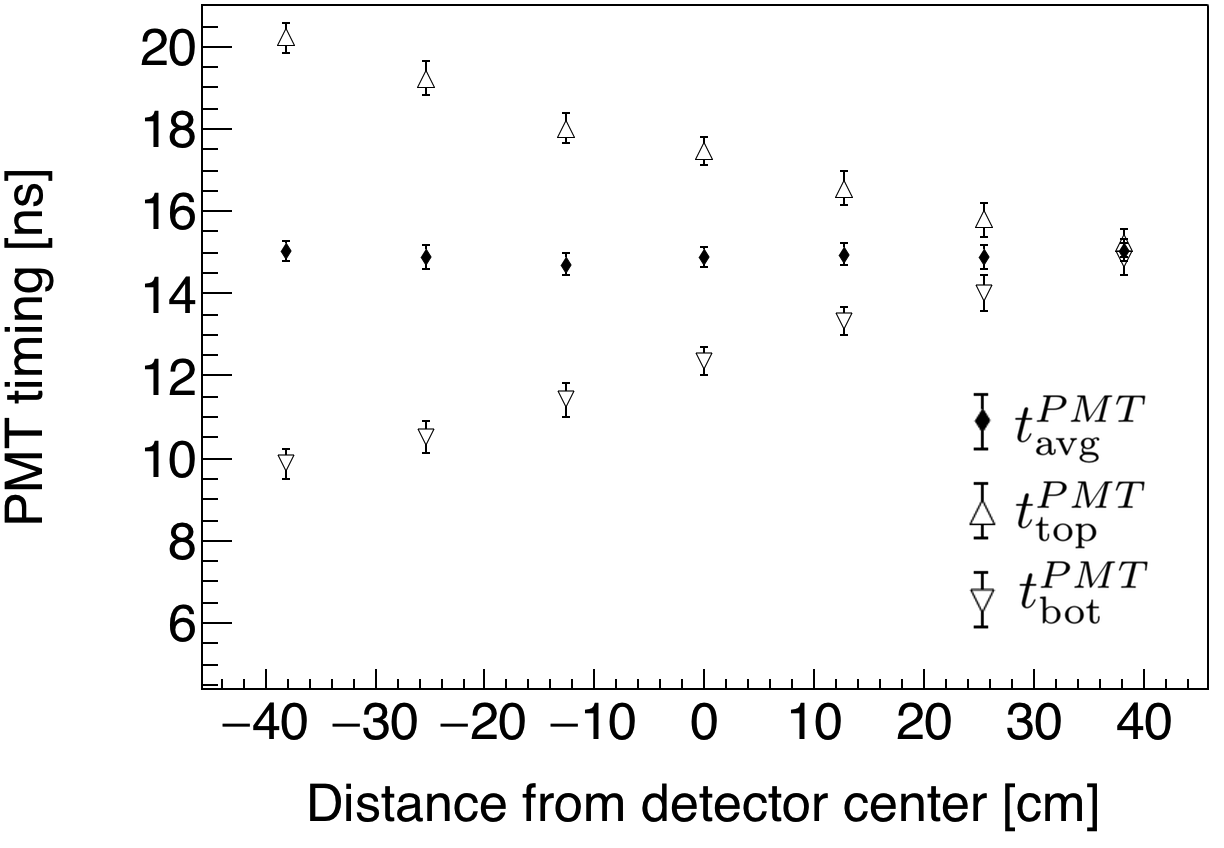
\includegraphics[width=0.6\textwidth]{Content/Methods/ConstPMTAvg.png}}

\subfloat[]{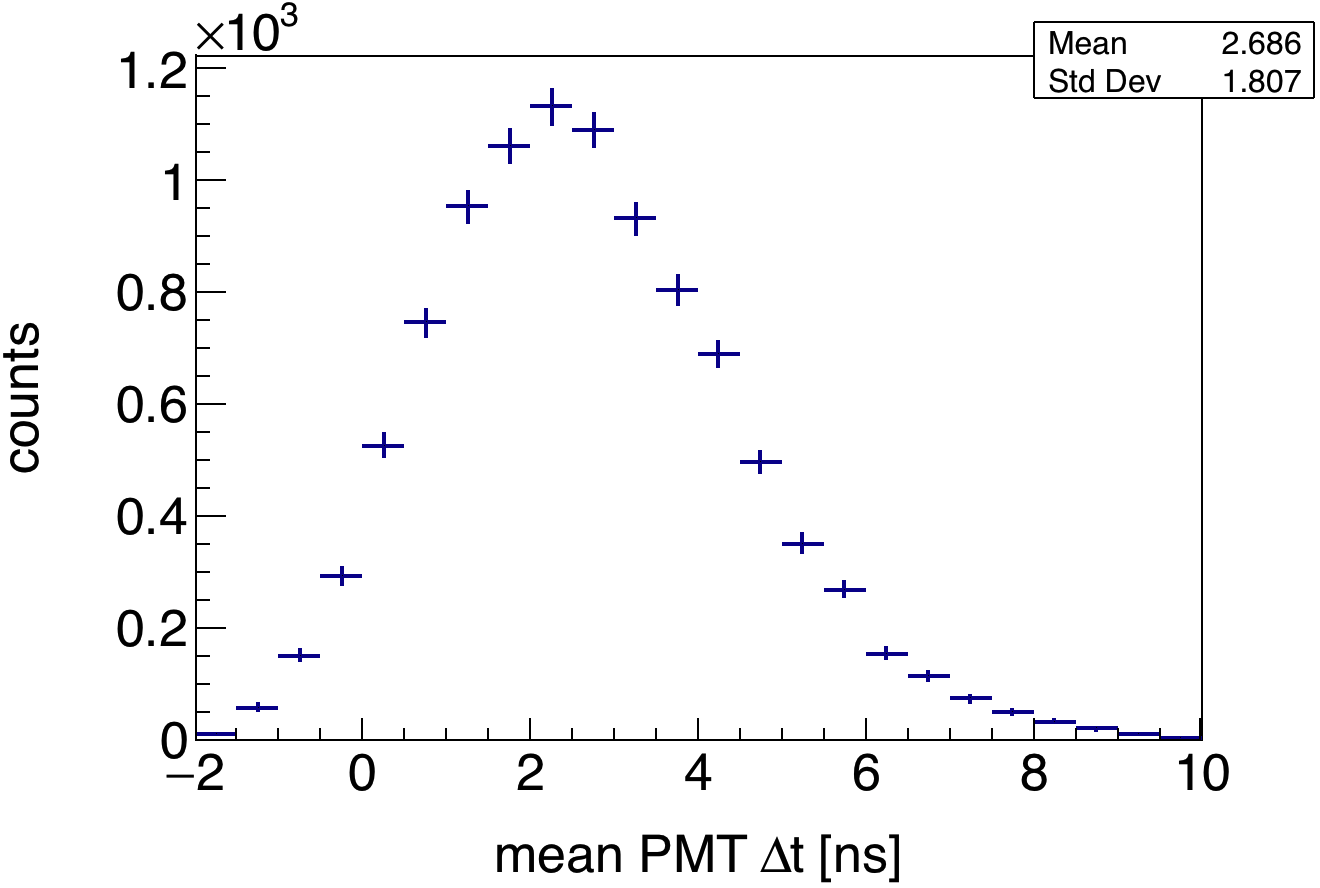
\includegraphics[width=0.6\textwidth]{Content/Methods/ConstPMTAvgProject.png}}
\caption{A collimated $^{60}$Co source is used to produce photon events with constant ToF at seven locations along the detector.
$^{60}$Co produces coincident photons, and one is detected by the scintillator and the other by a separate trigger detector.
 $\Delta t$ is the timing of a PMT signal relative to a signal from the trigger detector. 
 In (a), it can be seen that the average between signals from both PMTs does not depend on position.
By using the PMT average, there is a reduction in error due to the time required for scintillation light to travel through the scintillator.
The uncertainty in ToF measurements is equal to the standard deviation seen in (b), or about $\pm$2~ns, because all photons from the $^{60}$Co source have the same ToF.}
\label{fig:ConstPMTAvg}
\end{figure}

ToF is calculated by the following expression:
\begin{displaymath}
\text{ToF} = t^{PMTs}_{\text{avg}} - t_{\text{beam}} + C
\end{displaymath}
where $t^{PMTs}_{\text{avg}}$ is the average of the times of signals from both PMTs of a scintillator, $t_{\text{beam}}$ is the time of a signal provided by the accelerator at the beginning of each pulse, and $C$ is a constant timing offset determined by observing photons that scatter from the target.
Any process that produces a timing delay that does not change from pulse to pulse contributes to $C$, for example: \begin{itemize}
\item the time required for photons to travel from the bremsstrahlung radiator to the target
\item the propagation of signals through the wires connecting the PMTs
\item delays in the electronics
\item the signal transit time in the PMTs
\item the time required for scintillation light to propagate from the point of creation to both PMTs
\end{itemize}

The value of $C$ may be different for each detector, but this is not a problem because it can be determined accurately by comparing the timing spectra of the gamma flash of a non-neutron producing target made from aluminum, to the spectrum produced when no target is used.
The difference between no target and aluminum target reveals a prominent peak in the ToF spectrum due to photons that scatter from the aluminum target.
Photons which scattered from the target must travel between 125 cm to 130 cm before reaching the face of any detector, depending on whether the photons reach the detector near the center or at the top or bottom edge.
The two extreme cases are 125 cm and 130 cm distances, for which light takes 4.0~ns and 4.3~ns to travel, respectively.
The difference between these two times is negligible, so the ToF of photons that scatter from the target is assumed to be 4~ns.
This fact, along with the prominent photon peak seen in the timing spectra, is used to calculate the value of $C$ for each detector.

Under the assumption that neutrons travel to the detectors unimpeded, the calculation of neutron energy from ToF is straightforward.
This assumption is validated through MCNP simulations that tested the frequency of the scattering of fission neutrons within the target and the shielding of the detectors, and is discussed in sections~\ref{subsection:targets} and \ref{subsection:detectors}, respectively.
Figure~\ref{fig:ErgUncertainty}(a) shows the relationship between neutron energy and ToF, and Figure~\ref{fig:ErgUncertainty}(b) shows the measured neutron energy uncertainty according to the propagation of ToF measurement uncertainty through the calculation of neutron energy.
\begin{figure}[]
    \subfloat[]{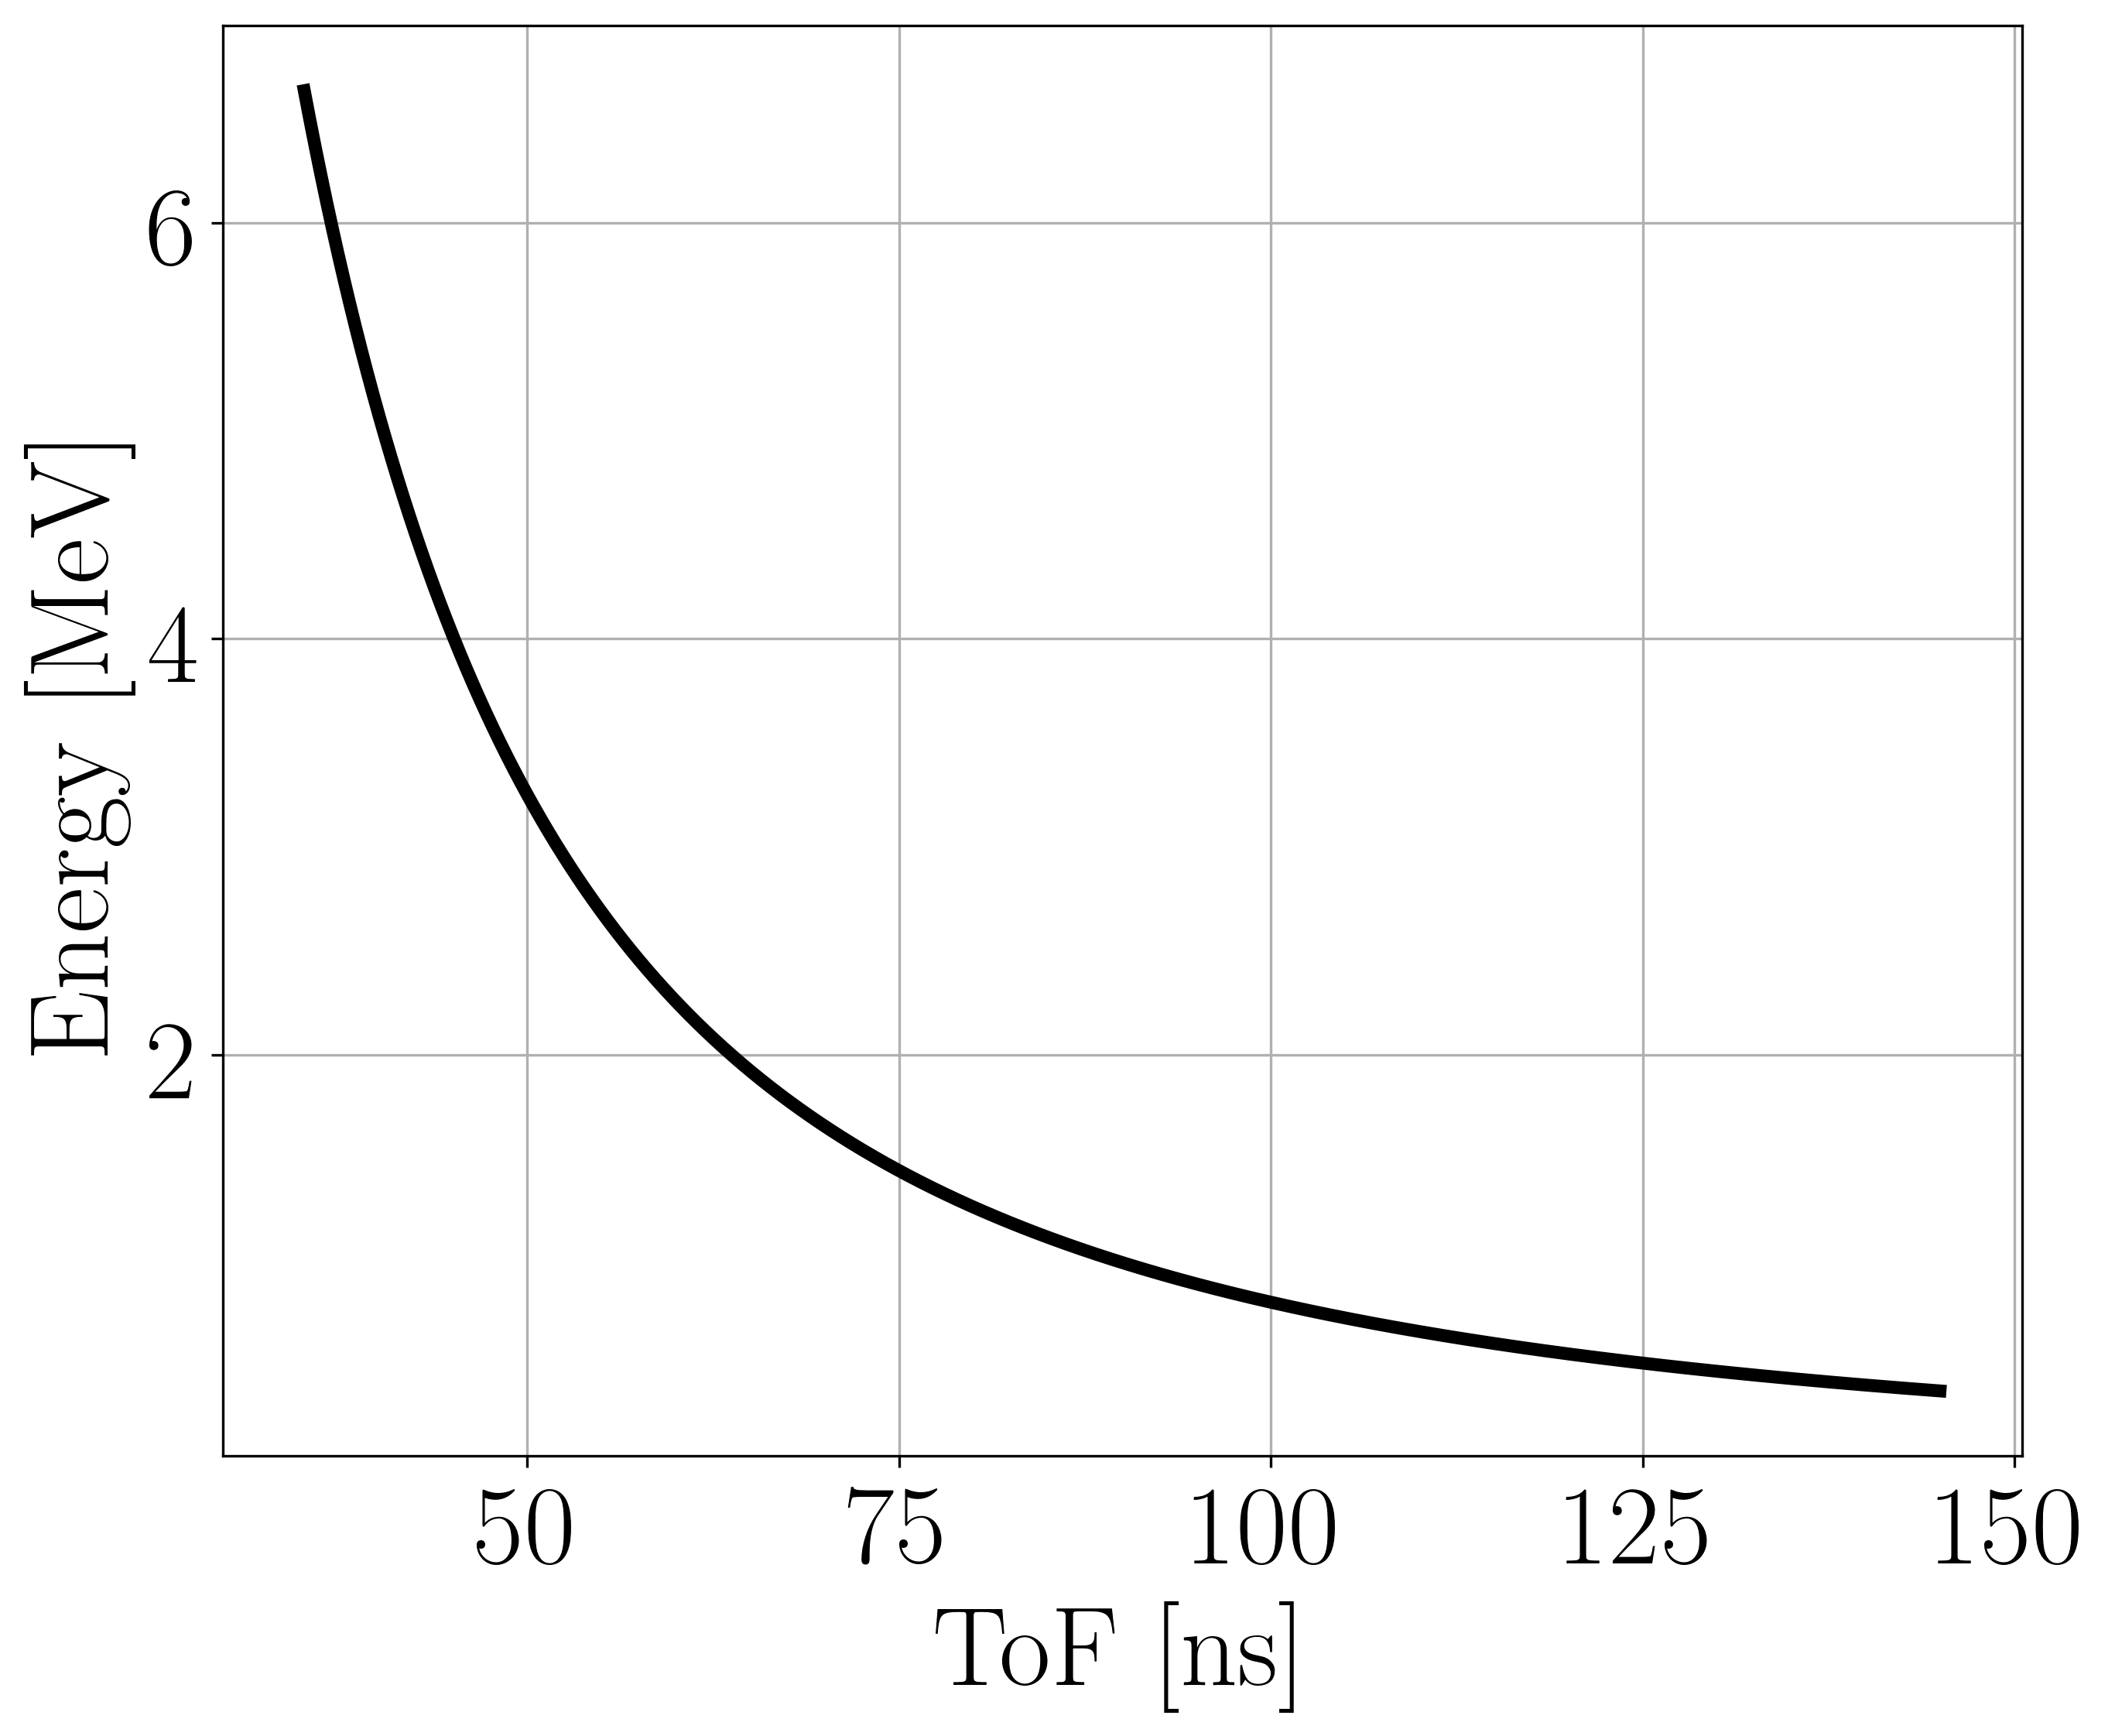
\includegraphics[width=0.5\textwidth]{Content/Methods/ToF2Erg.png}}
    \subfloat[]{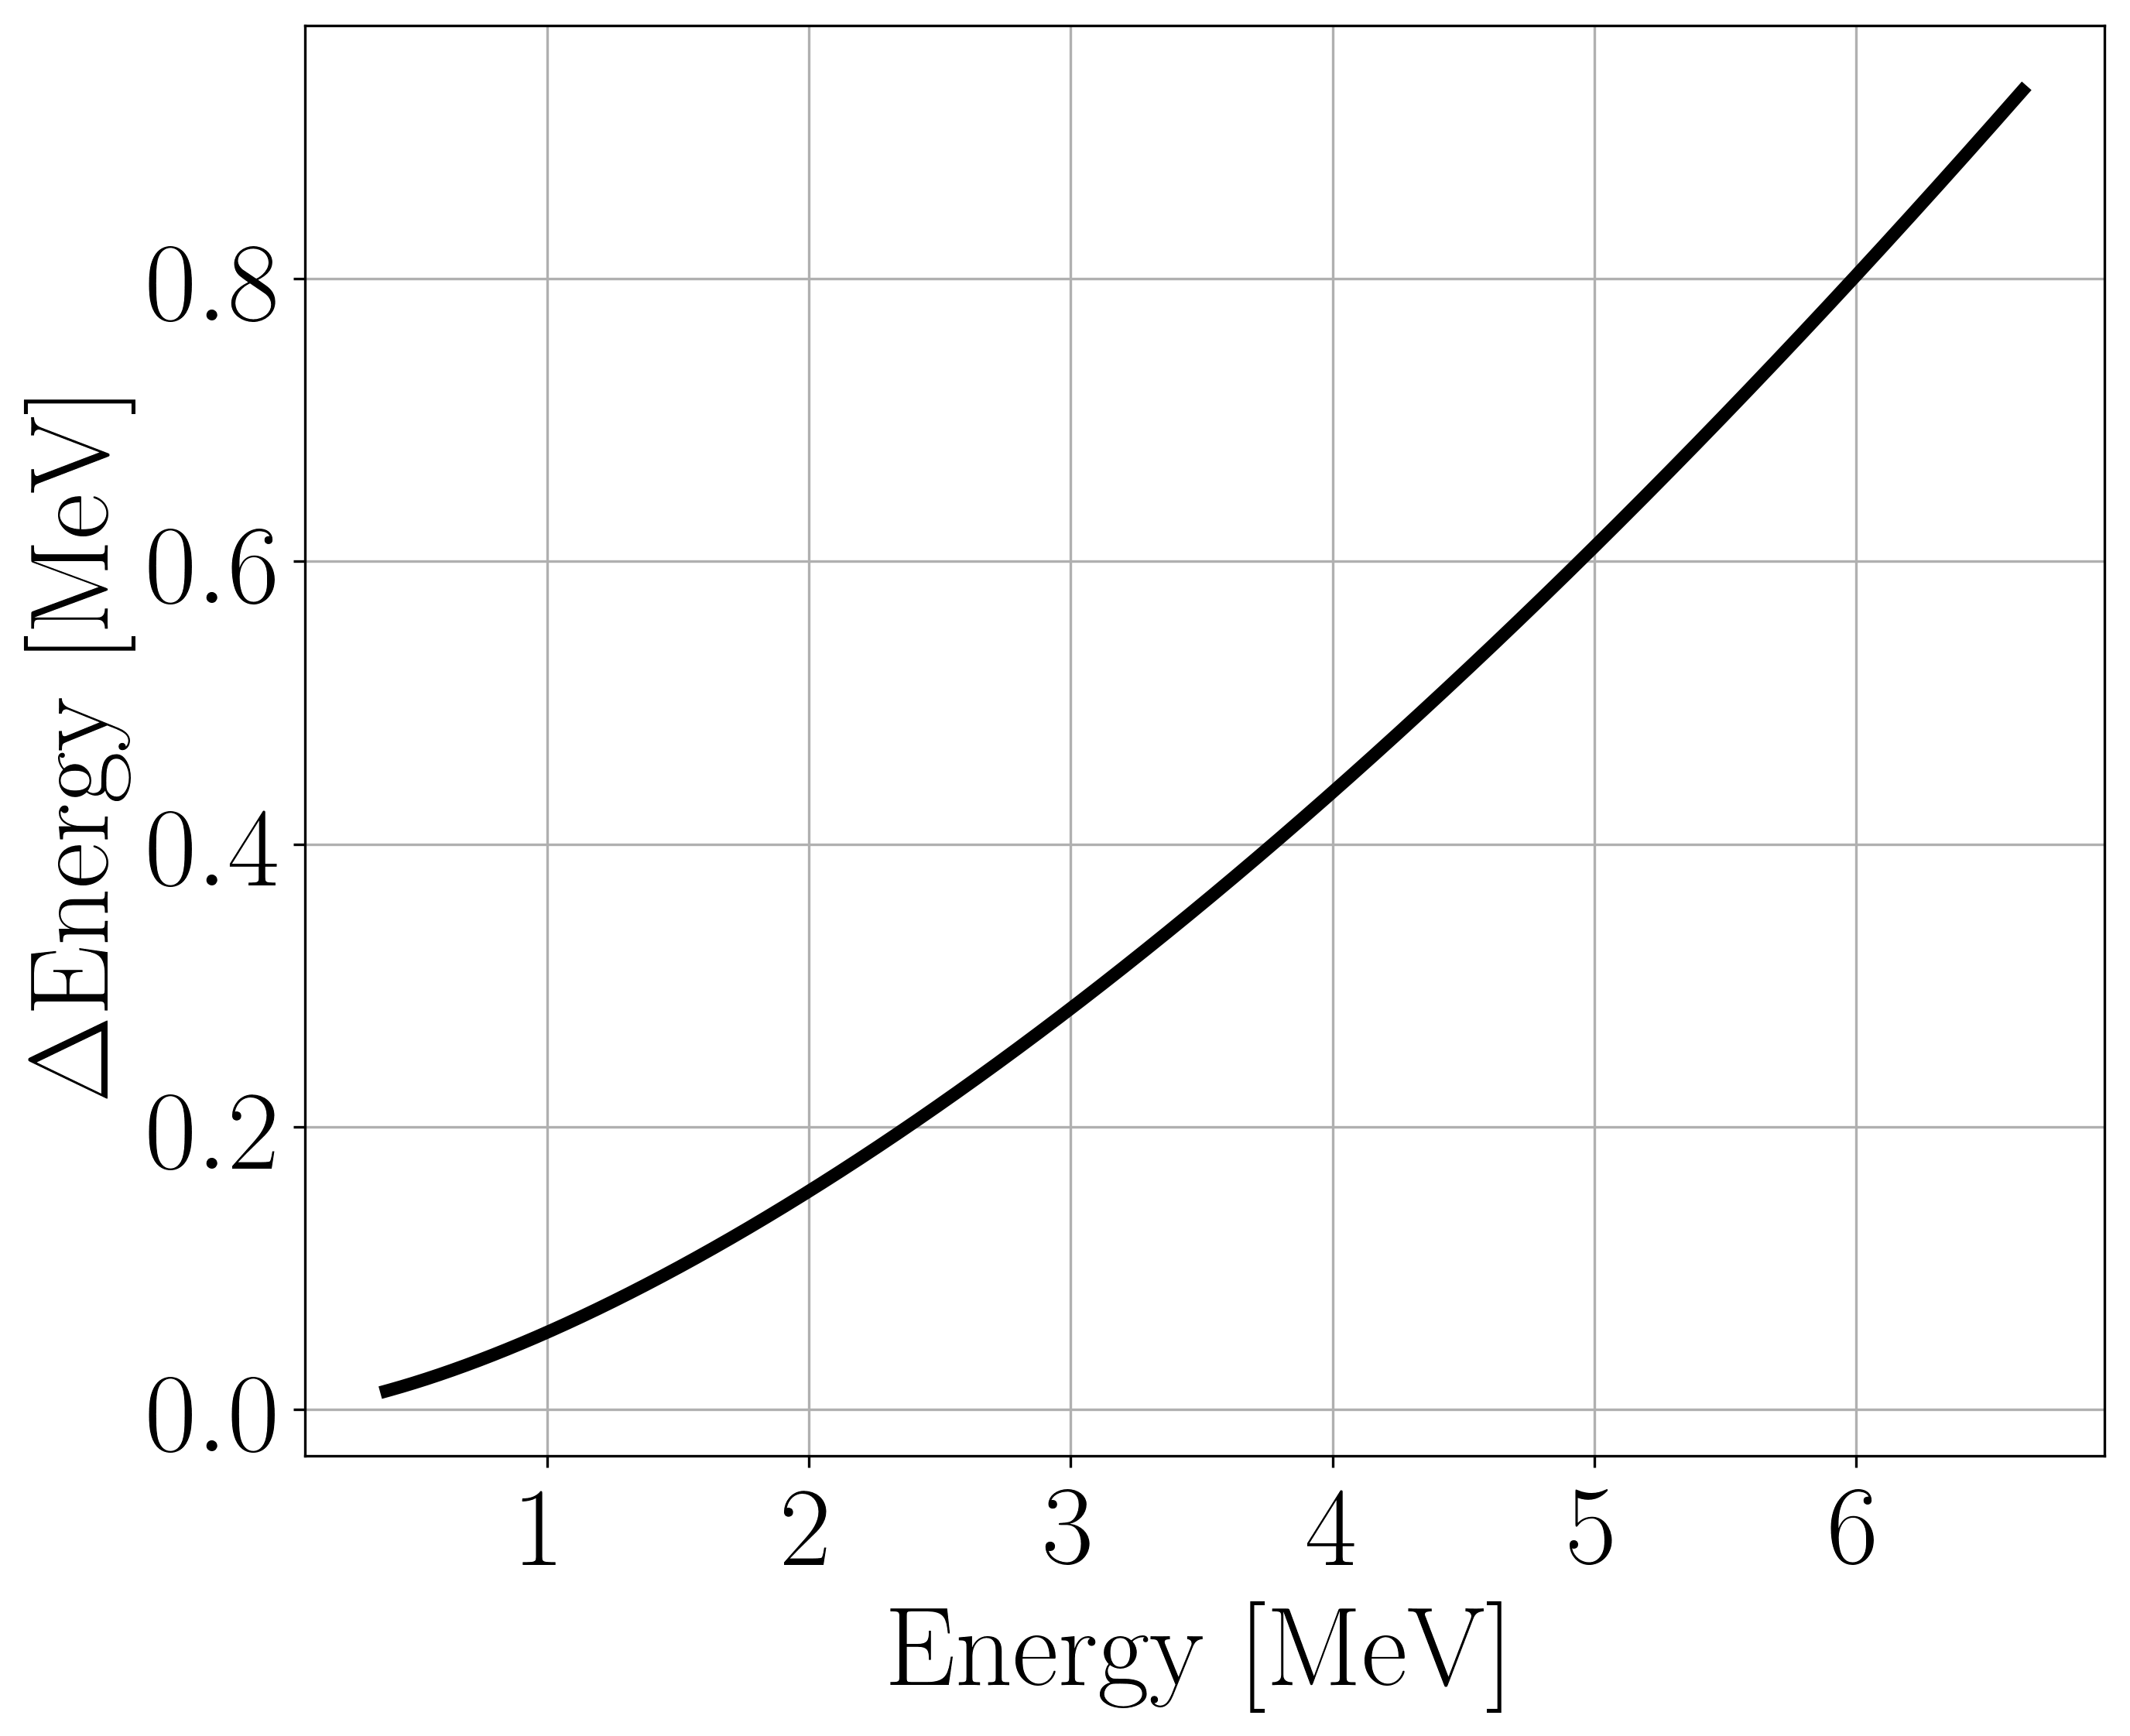
\includegraphics[width=0.5\textwidth]{Content/Methods/DeltaErg.png}}
    \caption{(a) Mapping from ToF to neutron energy: $E = \frac{8127}{ToF^{2}}$.
    (b) Uncertainty in neutron energy measurements as a function of measured neutron energy.}
    \label{fig:ErgUncertainty}
\end{figure}

\subsection{Particle Position Reconstruction}
The detectors are not capable of measuring the position of a detected particle along the axes parallel to the detectors' width (15.24~cm wide) and depth (3.81~cm deep), which contributes $\pm3^{\circ}$ to the total angular uncertainty.
The position of a particle hit along the 76.2~cm length of the scintillator is calculated using the timing difference of signals from both of a detector's PMTs.
Under the assumption that light travels at a constant velocity from some distance, $x$, relative to the center of a scintillator, the difference between the times of signals from the two PMTs, $\Delta t^{PMTs}$, is given by:
\begin{equation}
\begin{split}
\Delta t^{PMTs} & = t^{PMT_1}-t^{PMT_2} \\ 
& = \frac{(L/2 + x) n_{\text{eff}}}{c} - \frac{(L/2-x) n_{\text{eff}}}{c} \\
& = 2x \frac{n_{\text{eff}}}{c}  \, .
\end{split}
\end{equation}
Solving for $x$ gives 
\begin{equation}
\label{eq:position}
x = \frac{c}{2n_{\text{eff}}} \Delta t^{PMTs} 
\end{equation}
where $t^{PMT_{top}}$ and $t^{PMT_{bot}}$ are the times of signals from the top and bottom PMTs of a detector, $L$ is the length of the scintillator, $c$ is the speed of light, $n_{\text{eff}}$ is the effective index of refraction of the scintillator.
Using data taken from coincident photons from a collimated $^{60}$Co source placed at different position on a detector, a least squares linear fit between $x$ and $\Delta t^{PMTs}$ was performed.
The resulting fit parameters are used to find the position of detected particles.

The slope of the linear fit in Fig.~\ref{fig:PMTDifference}(b), along with Eq.~\ref{eq:position}, can be used to calculate the effective index of refraction, giving a value of 2.0 .
The index of refraction measured here is said to be ``effective" because its measurement is sensitive to scintillation light's speed only along the axis parallel to the scintillator's longest dimension, and because scintillation light does not necessarily take a straight path to the PMTs, this speed is not equal to the intrinsic speed of light in the material.
The actual index of refraction of PVT is known to be 1.58, or $\sim{20}\%$ less than the value measured here, indicating that there is some reflection of detected scintillation light from the boundaries of the scintillator.
This effect contributes to the width of the peaks in Fig.~\ref{fig:PMTDifference}(a).

\begin{figure}[]
    \centering
    \subfloat[]{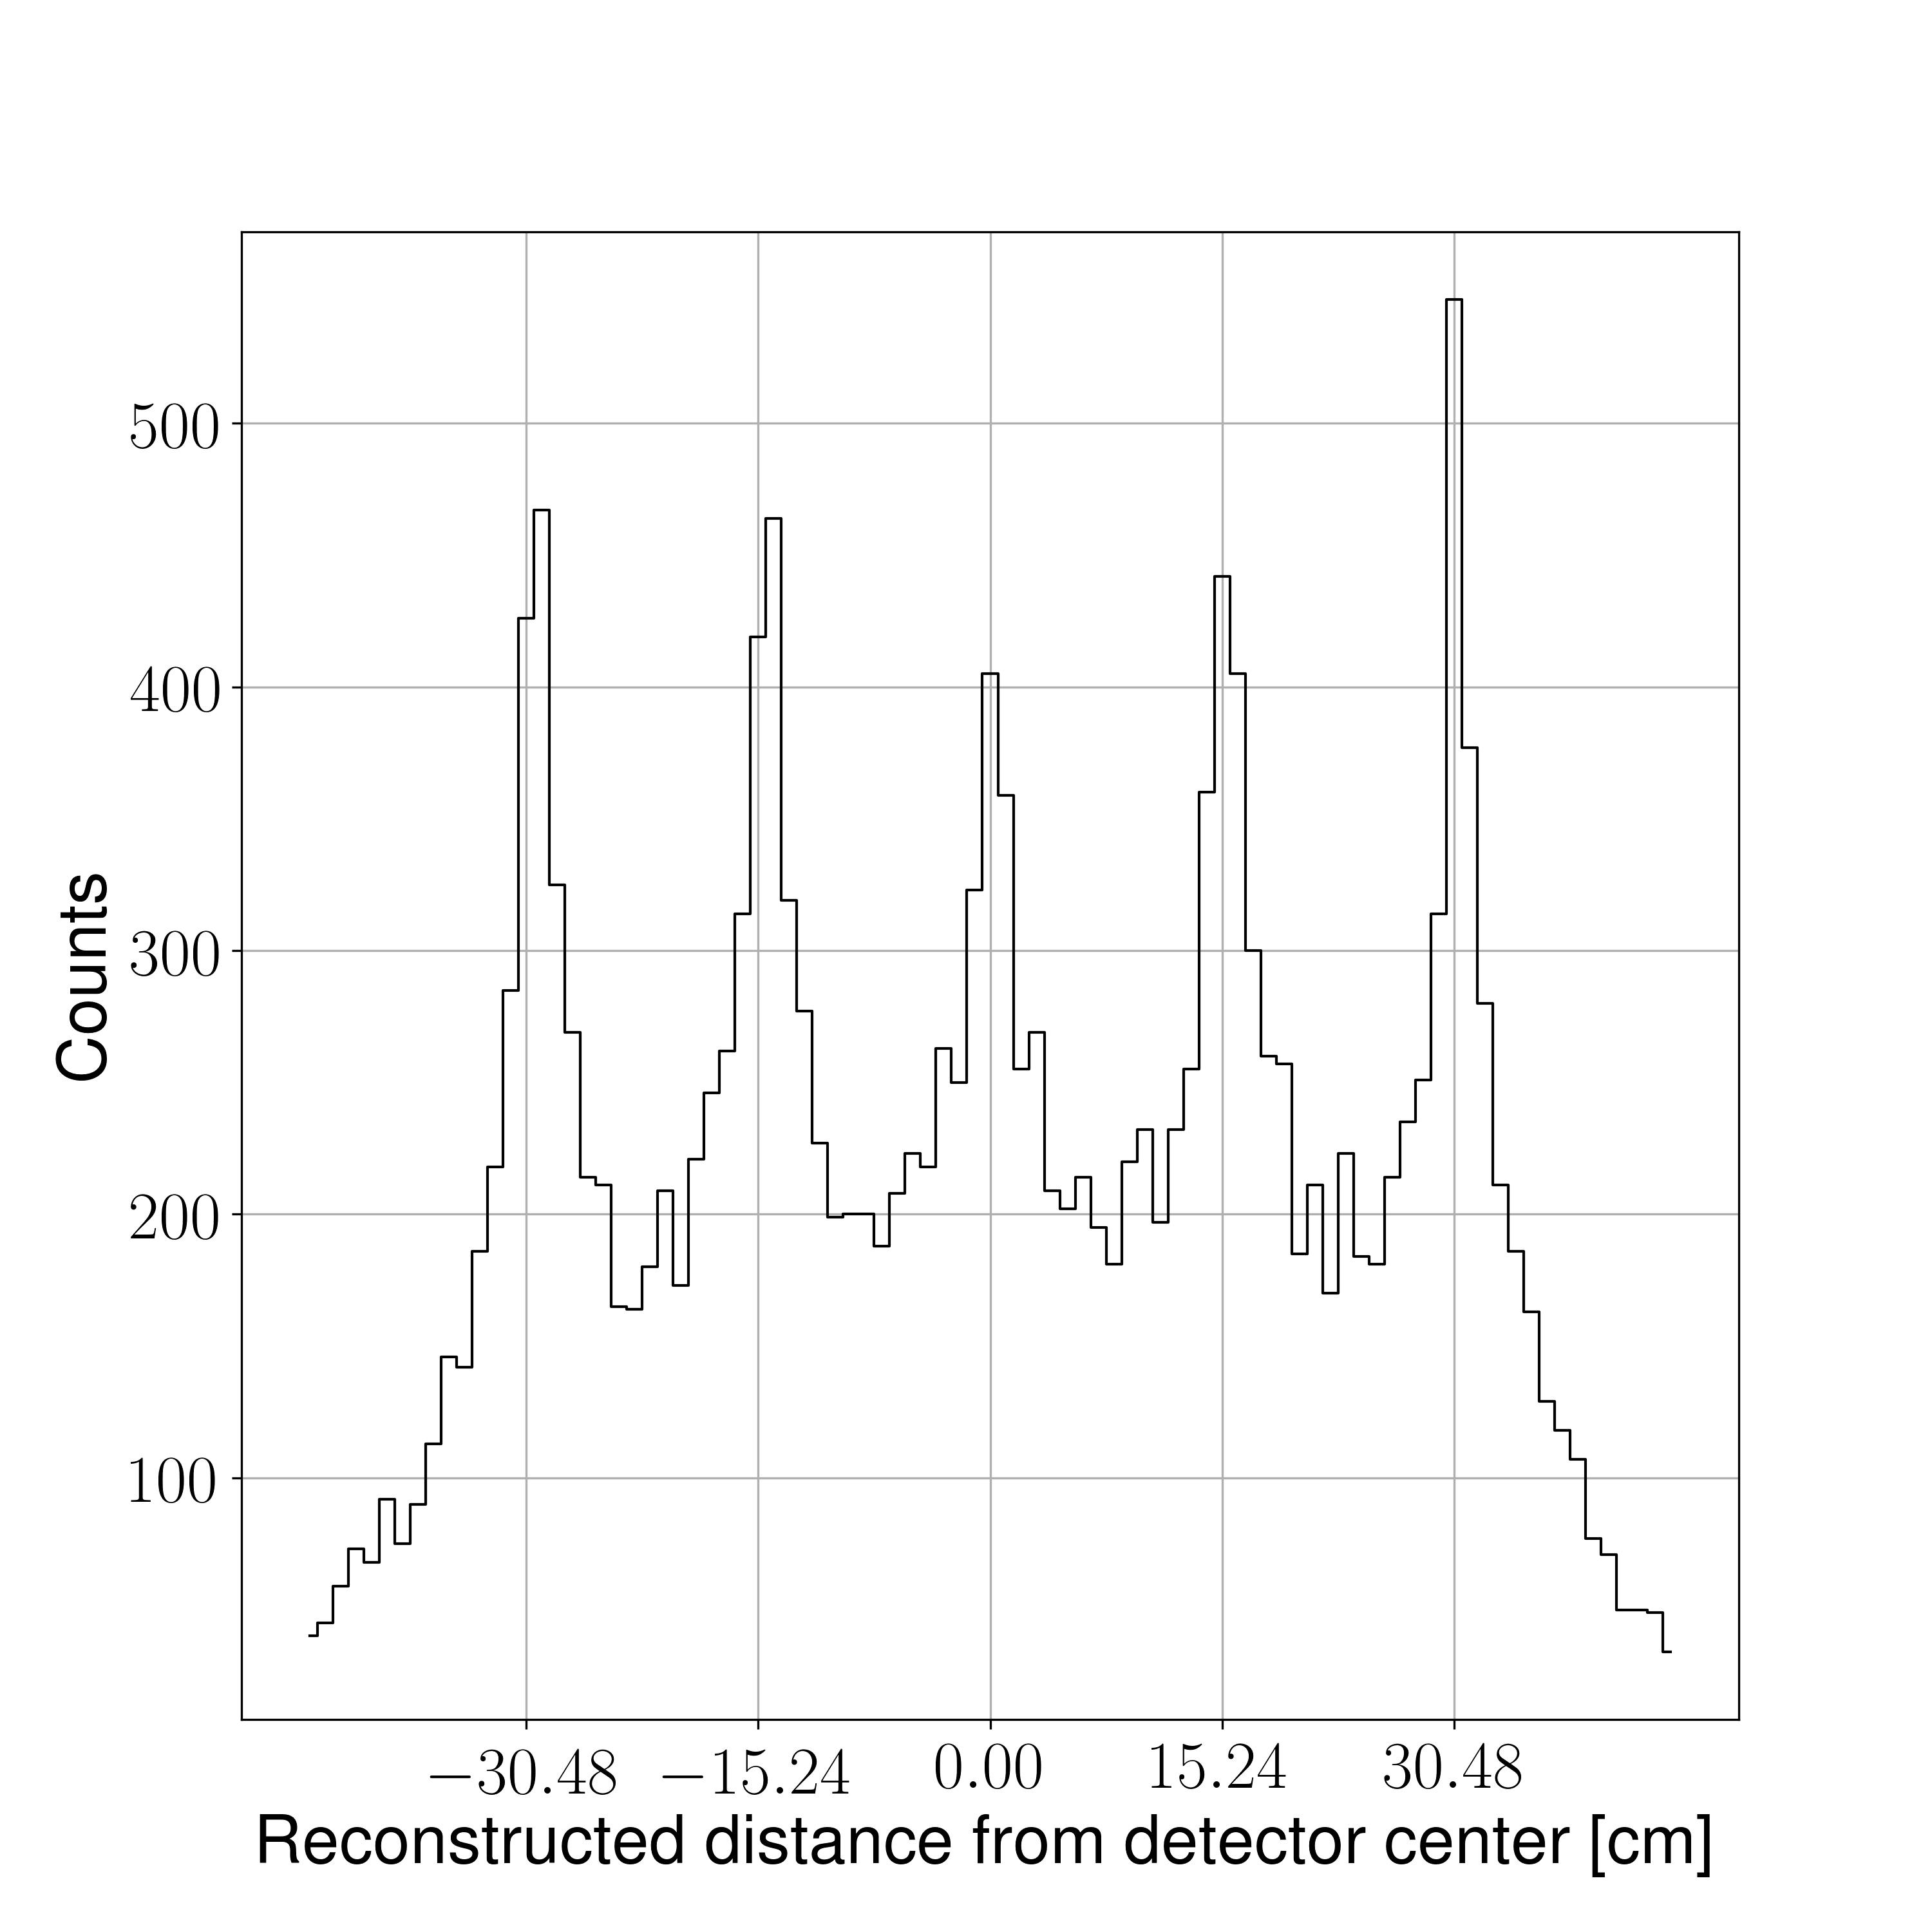
\includegraphics[width=0.6\textwidth]{Content/Methods/PMTDifference_hist.png}}
    
    \subfloat[]{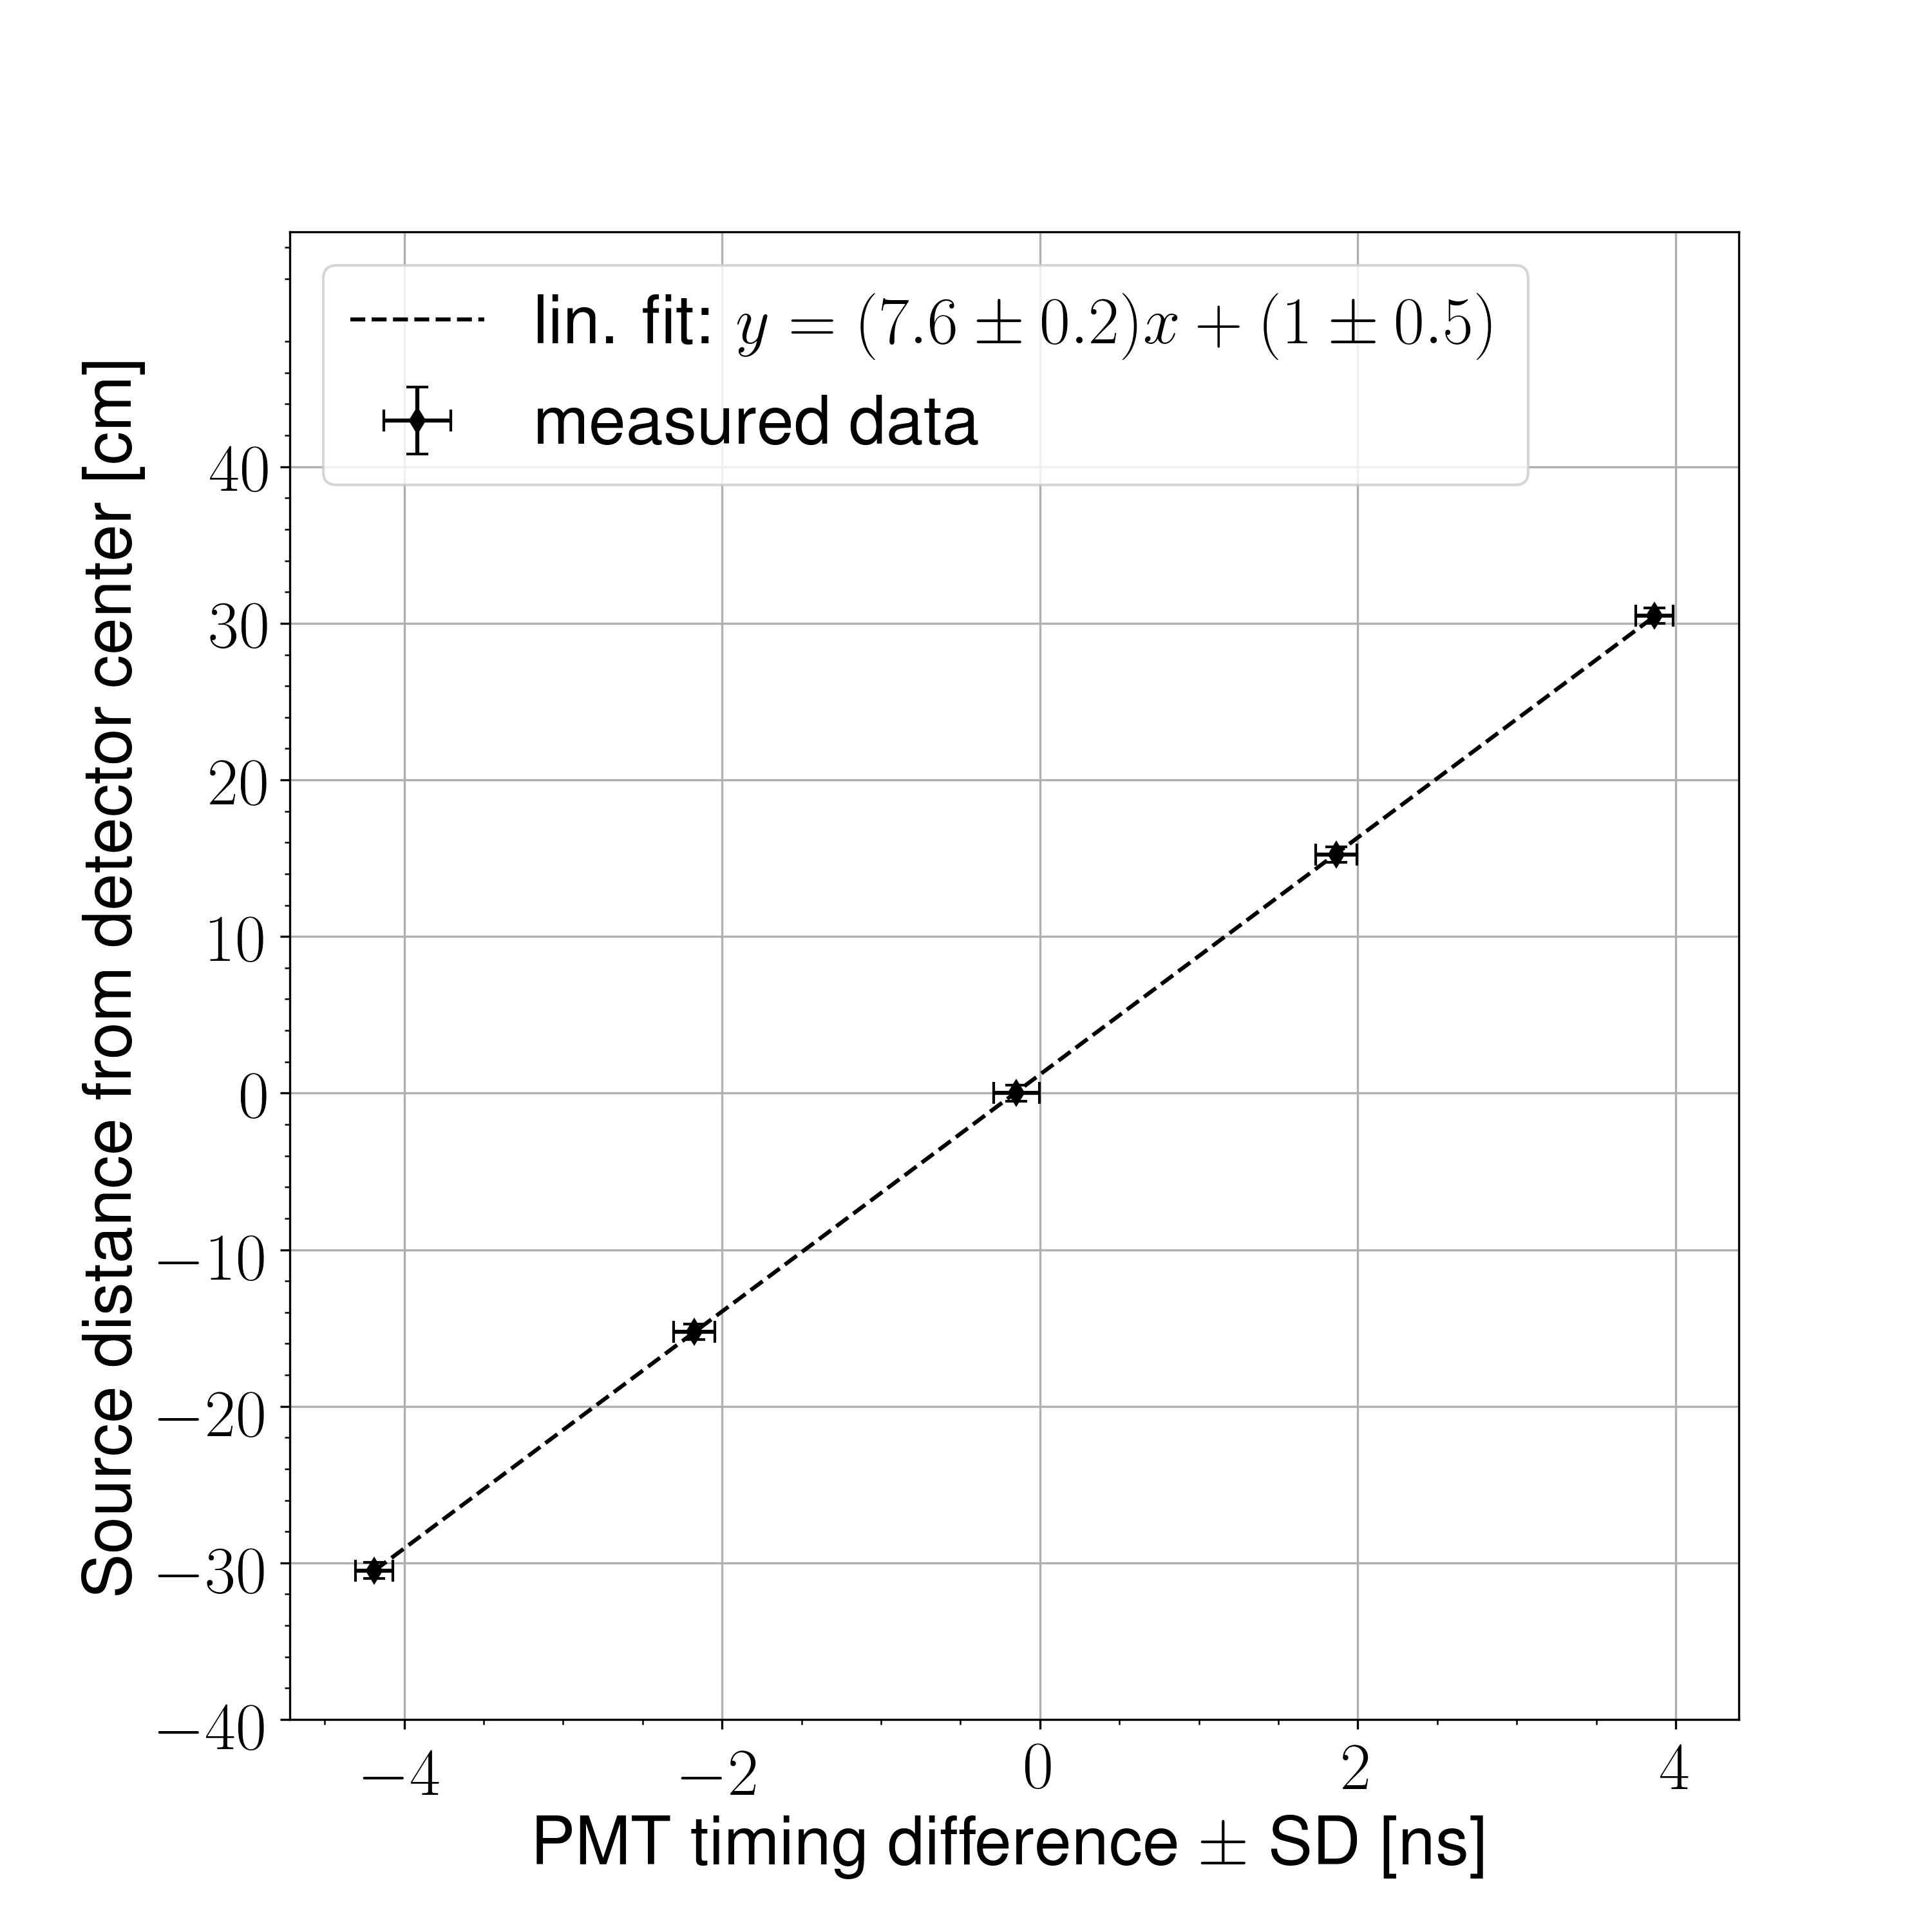
\includegraphics[width = 0.6\textwidth]{Content/Methods/PMTDifference.png}}

    \caption{
    A collimated $^{60}$Co source is used to produce photon events at five different positions along the scintillator with a spot size of less than 1~cm.
    Aggregating the data produces the five peaks seen in (a).
    The $\pm9$~cm width of each of these peaks is due to uncertainty in the measurement of particle position.
    As seen in (b), the mean PMT timing difference of events at each position varies linearly with respect to the distance of the $^{60}$Co from the center of the detector. 
    The result of a linear least squares fit to this data is used to calculate the position of detected particles along the scintillator.
    }
    \label{fig:PMTDifference}
\end{figure}

\subsubsection{Detector Shielding}
The detector's shielding was designed with the aim of reducing cross-talk, the detection of photons, and noise.
The front face of the detectors, facing towards the target, were subject to the highest gamma flux due to the scatting of the beam from the target.
The detection of a gamma renders a detector ``dead'' during the time at which subsequent fission neutrons from the same pulse reach the detector.
Lead can mitigate this problem by attenuating gammas, but has the side effect of scattering neutrons.
If a neutron scatters prior to being detected, the ToF calculation will be incorrect because the neutron traveled an unknown distance to the detector.
The extent that neutron travel distances are perturbed due to scattering from lead shielding was quantified using an MCNP simulation.
Accordingly, 1" of lead was placed along the front face of the detectors.
This diminished gamma detection rates to reasonable levels and, according to the simulation, caused a negligible amount of neutron scattering.
Because of the particularly high gamma flux, an additional 2" of lead was placed at the sides of detectors adjacent to the beam, and along the front faces of the detectors farthest downstream at $\pm30^{\circ}$ from the beam line.
Placing lead behind the detectors was avoided as an MCNP-POLIMI simulation predicted that lead placed here facilitates cross-talk.
Because cross-talk events are in fact correlated, they cannot be removed in analysis by the subtraction of accidentals.
For more information about cross-talk, see section~\ref{crosstalk}.

\subsection{Measurements with $^{252}$Cf}
\begin{figure}[h]
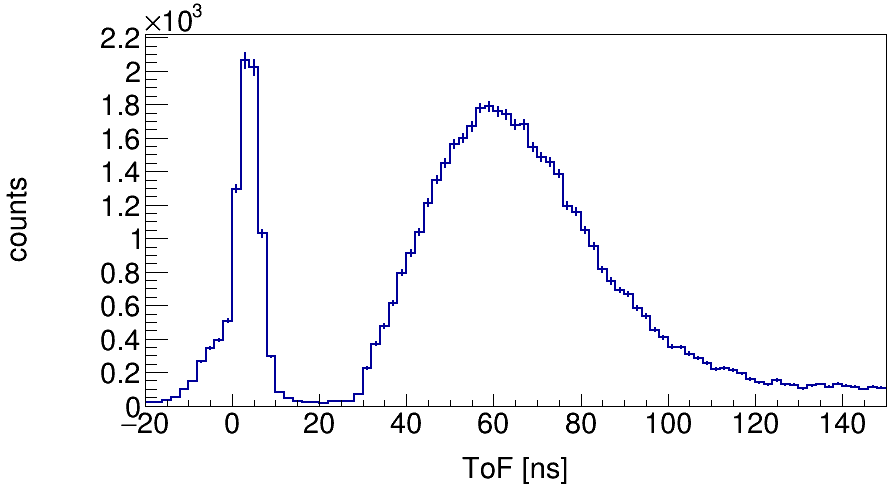
\includegraphics[width=0.9\textwidth]{Content/Methods/Cf252ToF.png}
\caption{Measured ToF spectrum from the SF of $^{252}$Cf.}
\label{fig:Cf252ToF}
\end{figure}
A $^{252}$Cf SF source was placed at the center of the detection system shown in Fig~\ref{fig:Facility} in order to measure two-neutron opening angle distribution.
Several such past measurements have been performed (see refs~\cite{1975Cf252, Pozzi2014, 2008CF252, Verbeke2018}), and thus they served as a means to validate the methods used throughout this study.

The $^{252}$Cf SF source produces a cleaner ToF spectrum than photofission due to the lack of a photon beam (see Fig.~\ref{fig:Cf252ToF}), and, therefore, the $^{252}$Cf measurements have a better signal to noise ratio.
Also, there is no concern over the detection of accidental neutron coincidences because the fission rate of the $^{252}$Cf source was about 3,500 fissions/s, making it highly unlikely that multiple fissions will occur during the electronic acceptance time window of 150~ns.
The beginning of the 150~ns time window was triggered by a 2-fold coincidence within a 4~ns window between two separate 10$\times$10$\times$5 cm$^3$ plastic scintillators, one placed above and the other below the source at a distance of 30~cm.
Aside from these differences in the time window triggering mechanism, identical methods were used for both photofission and SF measurements.